\chapter{twinX}

Una vez hemos analizado el material ya existente y desde el que partiremos para la construcción de twinX, vamos a ponernos manos a la obra con su desarrollo. Si bien es cierto que no se parte desde cero en cuanto a requisitos, sí que se va a reconstruir la herramienta desde cero, para poder aportar un gran significado a todos los módulos que vayan a formar parte de twinX y así podamos cohesionarlos de una mejor manera.

\section{Desarrollo de twinX}

Vamos a comenzar estableciendo las ideas principales del proyecto, reafirmando el propósito y viéndolo desde otras perspectivas que, aunque parecen obvias, no siempre se tienen en cuenta. Ello nos permitirá asentar las bases del producto software final y dotarlo de calidad.

\subsection{Diseño centrado en el usuario}

Esta disciplina, conocida también como \textit{User-Centered Design} o UCD, destaca por basar las fases del proceso de diseño estableciendo un enfoque constante en aprender del sujeto que utilizará el producto final. Es decir, para la consecución de los objetivos, es necesario tener una retroalimentación constante por parte del usuario final, que será quien vaya orientando nuestros avances según sea su interacción con lo que vayamos desarrollando.

El proceso dispone de unas fases a seguir, como son:
\begin{itemize}
	\item \textbf{Especificación del contexto de uso:} quiénes usarán el producto, para qué y bajo qué condiciones lo harán.
	\item \textbf{Especificación de requisitos:} identificar los objetivos que tienen que cumplirse para dejar a los usuarios satisfechos.
	\item \textbf{Crear soluciones de diseño:} en distintas etapas, desde un concepto poco definido hasta un diseño completo.
	\item \textbf{Evaluación de los diseños:} a través de las pruebas con los usuarios, de forma ideal.
\end{itemize}

\subsubsection{Pautas de Accesibilidad}

El no atender a causas de accesibilidad sería no aplicar correctamente, de alguna forma, el tipo de diseño escogido para el desarrollo del producto. Cuando se hacen pruebas, el objetivo no es otro que adaptar el producto para que pueda ser bien utilizado por el mayor número de usuarios posible y de la forma satisfactoria para ellos. Es por ello por lo que tenemos que abrir el abanico y contemplar que pueden ser numerosos los usuarios que necesiten adaptaciones para interaccionar correctamente con el contenido web.

Para ello, se propone la utilización de los recursos especificados en \textit{Web Content Accessibility Guidelines} (WCAG) \citep{wcag}. Con ello, podemos hacer que la experiencia en el sitio web pueda ser mínimamente satisfactoria para todo usuario que necesite hacer uso de la misma. En efecto, se deberán emplear una serie de técnicas, especificadas en su web, para que twinX sea adaptable. Entre ellas, destacamos la viabilidad de la interacción con el teclado, un texto descriptivo para las posibles imágenes que se puedan incluir, regular el contraste, etc. Con este proyecto, la intención es alcanzar el nivel AA (segundo más exigente), para que la gran mayoría de personas con necesidades especiales puedan usar la plataforma sin problema alguno.

\subsubsection{Encuesta SUS}

La encuesta SUS o \textit{System Usability Scale} es una de las encuestas que se pueden utilizar para evaluar la usabilidad de una cantidad de productos o servicios.

Sus únicos 10 enunciados es una de las cosas que más atractiva la hacen, puesto que hace que los usuarios la rellenen de manera rápida y fácil. También destaca por ser de denominación común y tener un bajo coste, además de poder corregirse inmediatamente después de terminar la encuesta. Es más, es una encuesta que puede aplicarse a casi cualquier tipo de interfaz de usuario, por lo que es muy versátil. Finalmente, cabe destacar la facilidad de entender los resultados, puesto que vienen dados en forma de una puntuación en el rango de 0 a 100.

Sobre los enunciado de la encuesta, tienen una escala de 1 a 5 cada uno, siendo 1 el indicador de mayor desacuerdo y el 5 el de mayor acuerdo. También se suele aportar unas pequeñas instrucciones a los candidatos a tomar la encuesta, indicando la necesidad de contestar todas las preguntas y de no pensarse mucho la respuesta a las mismas.

Para probar la eficacia de esta herramienta como elemento conductor en la creación de una interfaz de usuario a la hora de hacer pruebas y recibir \textit{feedback}, se hizo un experimento con una escala con adjetivos y no con números. Los resultados del análisis (\citep{sus}) vieron una mayor desviación de los resultados a la hora de expresar un mayor desacuerdo (adjetivos como «horrible» o «peor que lo imaginable» con números más próximos al 1). No obstante, en general, y gracias a análisis como el mencionado, se tiene evidencia que asegura que este tipo de encuestas es una buena herramienta a tener en cuenta a la hora de recibir información acerca de cuán bueno es nuestro diseño para los usuarios.

Por todo ello, esta será una de las herramientas que utilizaremos en las pruebas para constatar que los objetivos del proyecto se cumplen y cuáles pueden ser las conclusiones.

\subsection{\textit{Design Thinking}, DT}

El «Pensamiento de Diseño» o \textit{Design thinking} es una técnica de desarrollo que se centra en el usuario, pudiendo detectar y reaccionar ante cambios repentinos en el entorno de los usuarios y sus comportamientos. El objetivo está, mayormente, en abordar problemas con una pobre definición o que no se conocen a fondo para situar al usuario en el centro de todo y poder así enfocar el problema desde otras perspectivas, de manera que se pueda poner la atención en aquello que resulte de mayor importancia para los usuarios.

\subsubsection{Las fases del DT}

El proceso tiene unas fases no necesariamente secuenciales, de modo que puedan adaptarse lo mejor posible al proyecto, teniendo incluso la posibilidad de ejecutarse al mismo tiempo.

\begin{itemize}
	\item \textbf{Empatizar}, tratar de adoptar un conocimiento lo más empático posible del problema que se pretende resolver. Este es un elemento esencial, pues posibilita a los desarrolladores a descartar sus propias primeras conclusiones --erróneas a menudo-- y a entrar en materia con la realidad del cliente y sus necesidades.
	
	\item \textbf{Definir} las necesidades de los usuarios y sus problemas. Es la fase donde se reúnen y ordenan los elementos obtenidos como resultado de la fase anterior. A partir de entonces, se sintetizan para definir los problemas esenciales que se identifican, los cuales dan pie a la creación de \textit{personas}; esto es, la construcción de perfiles humanos en los cuales centrar el desarrollo.
	
	\item \textbf{Idear} y hacer frente a lo que se da por hecho, creando formas alternativas de ver y tratar el problema con soluciones innovadoras, a partir de lo estudiado en las dos fases anteriores.
	
	\item \textbf{Prototipado} de las soluciones pensadas, una fase experimental cuyo objetivo es el de encontrar la mejor solución para cada uno de los problemas encontrados. Los desarrolladores han de producir una versión de bajo coste del producto para investigar cuál es el resultado de haber llevado las ideas a la práctica.
	
	\item \textbf{Pruebas} con lo obtenido, para analizar si realmente se ha llegado a un buen resultado o, si por el contrario, se ha de retroceder a otra fase para redefinir uno o más problemas.
	
\end{itemize}

Como hemos indicado, las fases no siempre siguen el mismo orden. Hay veces que se toman decisiones como la de saltar de la primera fase de empatía a la penúltima de prototipado, probablemente para aclarar las ideas y poder hacer una mejor definición, a través de la muestra de material al cliente que pueda animarlo a dar una mayor retroalimentación. Del mismo modo, si el prototipado no ha ido bien, se puede volver a la tercera y anterior fase, la de construcción de ideas. Incluso podría darse el caso que haciendo pruebas, los desarrolladores nos demos cuenta de que no se ha llevado a cabo una buena ejecución del proceso y sea preciso volver a la segunda etapa de definición de los problemas. Siempre es mejor ir hacia atrás en lugar de comenzar la casa por el tejado, así que toda maniobra que sea apropiada para una mejor construcción del producto y que lo dote de calidad siempre es bienvenida.


\subsubsection{Herramientas del DT}
\label{herramientasDT}

Hay una serie de actividades o técnicas que nos pueden resultar útiles para llevar a cabo el trabajo de desarrollo con eficacia y que suelen tener éxito. Destacamos las siguientes:

\begin{itemize}
	\item \textbf{Creación de personas:} perfiles ficticios de los distintos usuarios que utilizarán el producto software. Creadas en la fase de definición, no solo se especifica el propósito específico de interacción con el producto a mejorar o la necesidad por que exista el software que se quiere desarrollar. Describimos el contexto del personaje, sus inquietudes y, en definitiva, lo que hay detrás de esa persona en más ámbitos que puedan ayudar a comprender por qué es necesario que se tengan en cuenta ciertas cosas a la hora del desarrollo.
	
	\item \textbf{\textit{Brainstorming}:} también conocida como nube de ideas que radican alrededor de un concepto central. Se trata de escribir conceptos que vengan a la cabeza de los intervinientes en la creación del esquema, sin importar los análisis o el futuro que puedan tener en el proceso. Cualquier cosa que tenga que ver con lo que se está tratando es válida, pues lo que aparentemente resulta absurdo podría en muchos casos resolver parcialmente el problema o ayudar a enfocarlo. Así, cuantas más propuestas, mejor se lleva a cabo este proceso, que tiene lugar en la fase de ideación.
	
	\item \textbf{Prototipado en papel:} la creación de prototipos (en la cuarta fase de prototipado) con un material del que todos disponemos es extremadamente sencilla a la par que útil. Cuando las cosas se plasman en un folio, podemos apreciar matices que no nos venían a la cabeza cuando la idea era tan solo un concepto. Si bien es cierto que depende de las dotes artísticas de la persona que dibuja el prototipo, el hacerlo con papel y lápiz ayuda a volcar la concentración de una manera diferente a como se hace cuando se programa o se diseña con herramientas informáticas.
	
	\item \textbf{Mapas de experiencia de usuario:} también conocidos como \textit{Customer Journey Maps}, sirven para representar la experiencia de un usuario a lo largo del tiempo. En ellos plasmamos la forma en que un diseño cubre o no las necesidades de un usuario utilizando un producto o servicio. Es justo por eso por lo que estos mapas han de ser lo más descriptivos posibles, representando con gran detalle las acciones y subtareas que tiene que desempeñar un usuario al usar el sistema.
	
\end{itemize}

\subsection{Aplicación de las metodologías}

En relación con las fases del DT, podemos diferenciar a través de las cuales ya hemos ido pasando. El comienzo del proyecto vino acompañado de una serie de reuniones que se incluyen en los anexos. En este contexto, la fase de \textbf{empatización} se correspondería con las dos primeras reuniones, donde se establecieron un primer contacto y las bases del proyecto, atendiendo al testimonio de los usuarios reales de TWINS, lo que actualmente se está usando para resolver los problemas a los que se tienen que enfrentar en la ORI-FyL. Es más, en la segunda reunión (~\ref{reunion2}) se habló de algunas características ideales y que está costando implementar en el actual escenario, lo que podríamos englobar dentro de la \textbf{ideación}. Por último, ya en la tercera reunión, se tiene la \textbf{definición} de todos los conceptos necesarios para comprender el funcionamiento de TWINS y de la oficina en general. No obstante, a lo largo de esta sección, vamos a continuar esta fase con la definición de más elementos necesarios para llevar a cabo el desarrollo de twinX.

Con esas tres fases cubiertas, se puede dar comienzo a las otras dos: la de \textbf{prototipado} y \textbf{pruebas}, que serán desarrolladas de forma más extensa en las secciones ~\ref{bocetos} y ~\ref{pruebas}. %PENDIENTE: comprobar referencias, ya que han sido puestas antes de tiempo y añadir posibles futuras reuniones y sesiones de pruebas.

\section{Personas ficticias}

Tal y como hemos comentado en la sección \ref{herramientasDT}, una de las herramientas que nos permiten definir el alcance y las necesidades de la aplicación es la creación de perfiles de personas ficticias, candidatos a utilizar twinX en un futuro. De esta forma, tanto por la parte del desarrollo como por la del interesado en el producto final, pueden no solo hacerse una mejor idea de los objetivos del mismo, sino también justificar su creación.

Vamos a tratar de crear tres personalidades lo más variopintas posibles en aras de enfocarnos más aún en el usuario y dotar de mayor calidad el resultado final, de modo que podamos abarcar por completo el entorno de influencia del problema. (Herramienta: \citep{uxpressia})

\begin{figure}
	\centering
	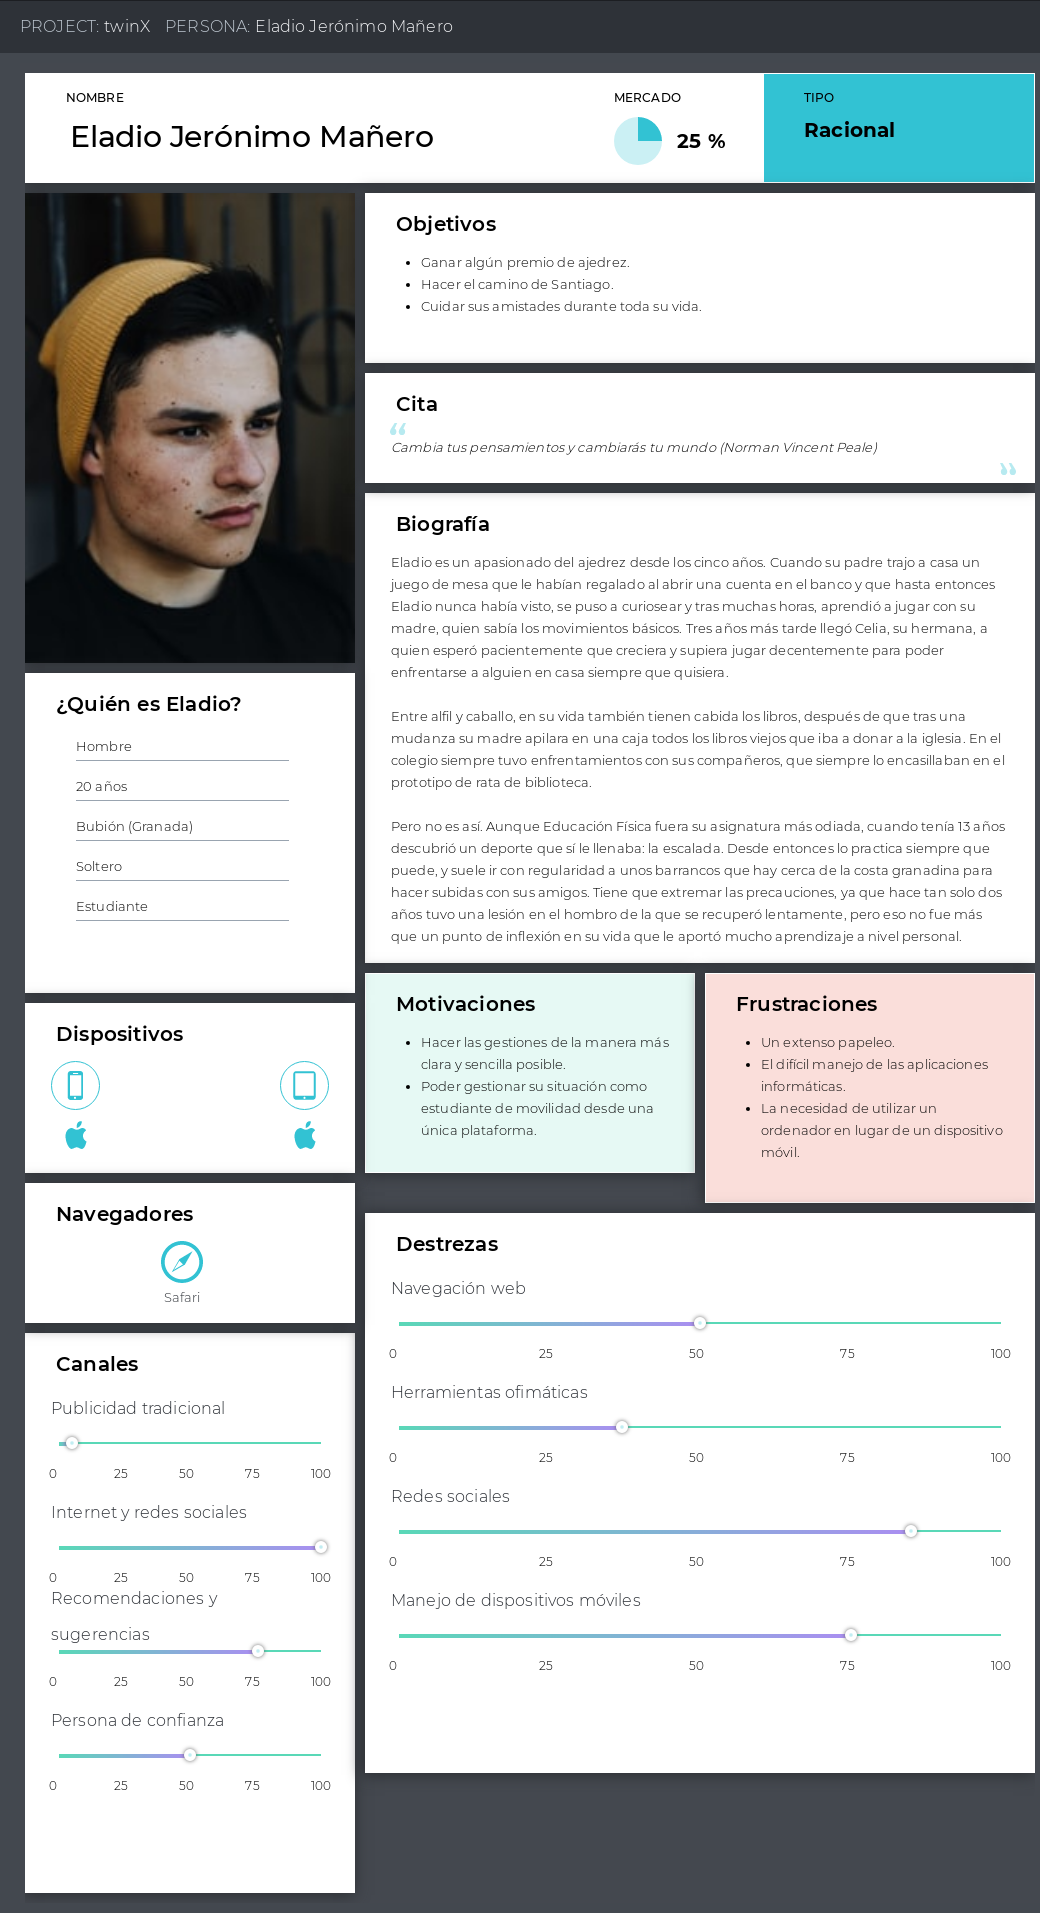
\includegraphics[width=\textwidth, height=\textheight, keepaspectratio]{img/Personas/Eladio}
	\caption[Persona \#1]{Persona \#1: Eladio}
	\label{fig:persona1}
\end{figure}
\begin{figure}
	\centering
	\includegraphics[width=\textwidth, height=\textheight, keepaspectratio]{img/Personas/MGracia}
	\caption[Persona \#2]{Persona \#2: María Gracia}
	\label{fig:persona2}
\end{figure}
\begin{figure}
	\centering
	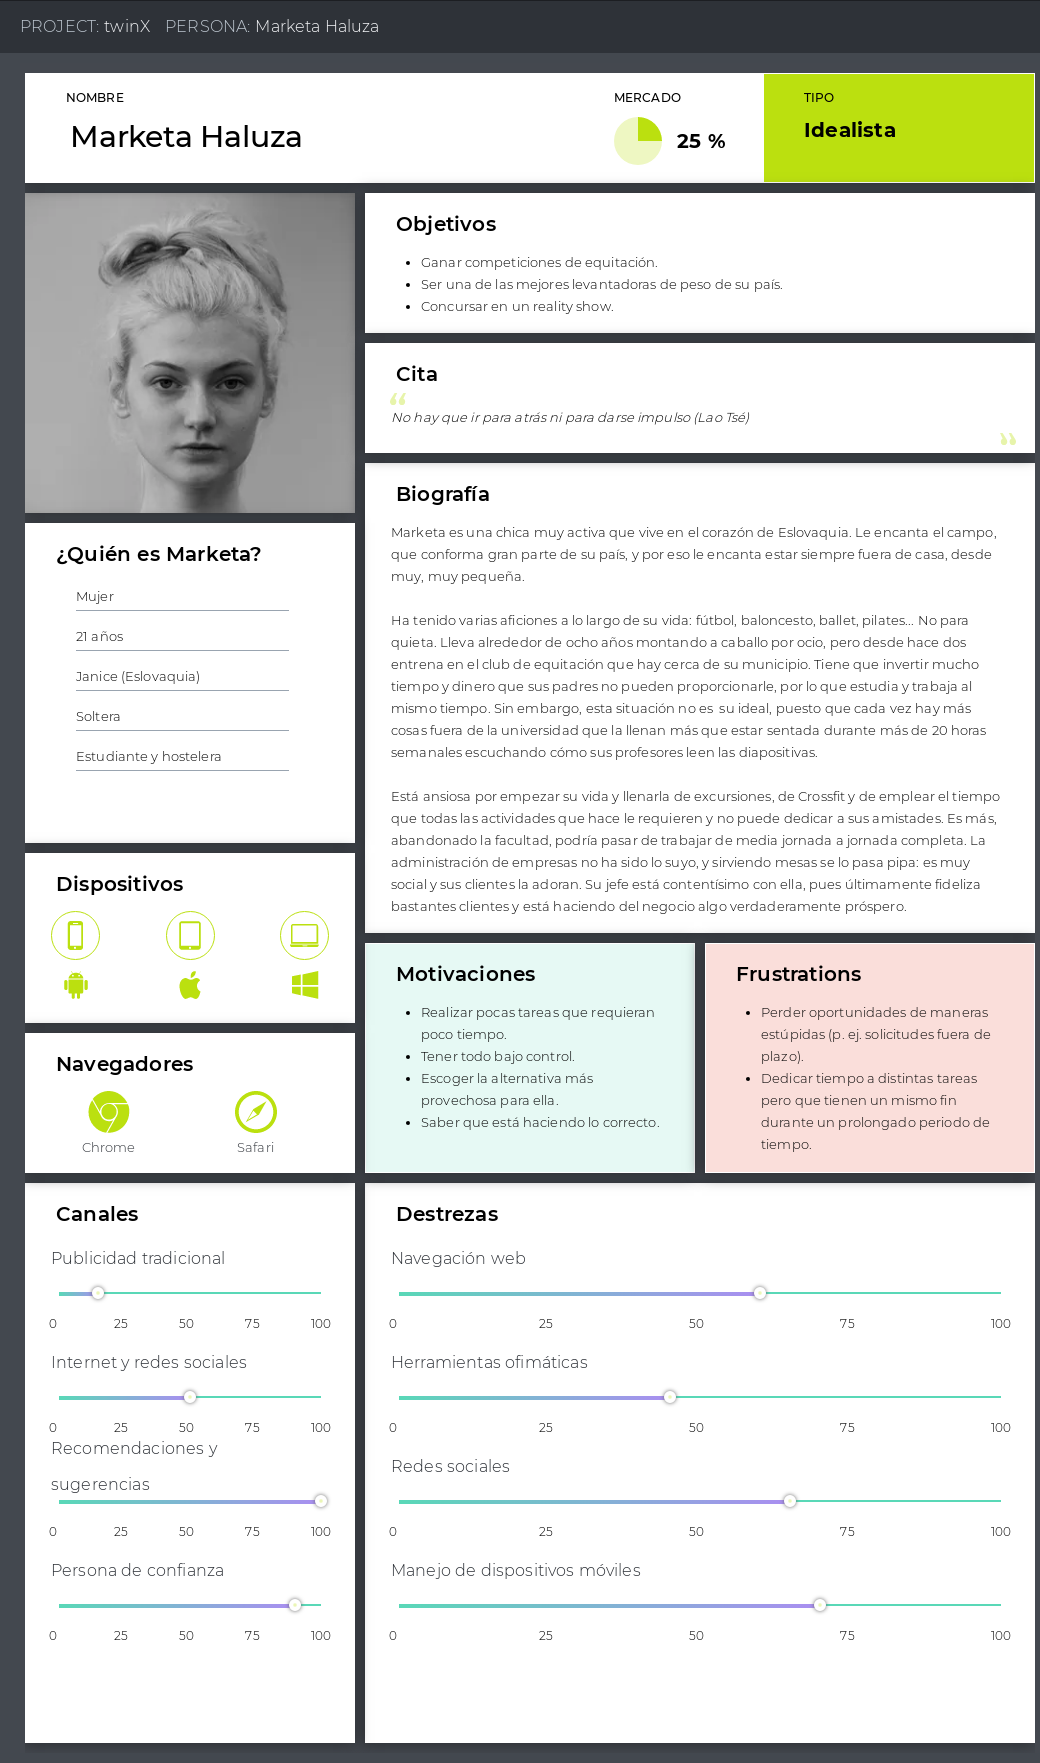
\includegraphics[width=\textwidth, height=\textheight, keepaspectratio]{img/Personas/Marketa}
	\caption[Persona \#3]{Persona \#3: Marketa}
	\label{fig:persona3}
\end{figure}

En vista de la persona en la figura \ref{fig:persona1}, Eladio, podríamos pensar que para él, lo óptimo sería desarrollar una app móvil para poder gestionar su movilidad, en caso de que quisiera hacerla. Pertenece a las nuevas generaciones donde apenas se usa el ordenador, hasta llegar a la universidad, mayormente, por lo que está acostumbrado a una tablet. Al mismo tiempo, María Gracia (figura \ref{fig:persona2}) trabaja gestionando información como la de estudiantes como Eladio o Marketa (figura \ref{fig:persona3}) y no puede permitirse interaccionar con un dispositivo móvil, pues tardaría mucho en realizar su trabajo, y no lo haría de forma efectiva. Por tanto, una solución web parece una resolución del problema apta para la mayoría del mercado del producto.

Como decíamos, nos sirven elementos que no tengan que ver directamente con las habilidades tecnológicas de los candidatos; y es que, por ejemplo, María Gracia en este caso no podría tampoco ver una web que no tuviera la tipografía lo suficientemente grande como para leer, porque podría tener la vista cansada. O quizás Marketa, si no tiene una buena situación económica, tendría quizás que conectarse desde un dispositivo algo obsoleto, por lo que probablemente le sea muy costoso en cuanto a tiempo cargar una página web con numerosas imágenes.

En definitiva, podría pensarse que los perfiles de estas tres personas están hechos para hacer el análisis de cualquier aplicación o producto software, ya que no hemos ideado estas personalidades específicamente para el problema que nos compete. Es por ello por lo que podemos tomar estos perfiles ficticios como válidos, pues no están «hechos a medida» para nosotros. Gracias a ello, podemos adaptar el desarrollo a una serie de necesidades y/o conflictos que pueden generar en otras personas al mismo tiempo, obligándonos a buscar una solución homogénea para todos, funcional y, no menos importante, que resuelva el problema como es debido y dadas las necesidades.

\section{Entrevistas}

Las reuniones con las personas que pueden entenderse como «el cliente» del producto software, han sido esenciales para el desarrollo del mismo. En primer lugar, se establecieron las bases y se definieron los problemas. Una vez lograda la comprensión, nos pusimos manos a la obra a definir cómo podríamos abordar el problema de forma que se pudiera aportar una solución de valor; si bien no definitiva y que resolviera el problema por completo, pero sí un buen comienzo como pretendemos alcanzar con este proyecto.

Como decimos, el valor de las reuniones es muy alto. Sin ir más lejos, dependía de la interacción con el creador de TWINS, Miguel Ángel Sanz, de la comprensión de los procesos implicados y de la cesión del acceso al material para la realización del proyecto. No de menos importancia son las reuniones utilizadas para la realización de pruebas, ya que durante el proceso de desarrollo el enfoque estaba en simplificar y tratar de plasmar el núcleo de TWINS para construir twinX, lo que podría llevar a futuros problemas de conceptos o de carencias no detectadas a tiempo, para lo que es fundamental el contacto con los verdaderos usuarios finales de la aplicación --o al menos en sus primeras fases--.%PENDIENTE REVISAR LO QUE SE DICE O LO QUE FALTA DE LAS ÚLTIMAS REUNIONES DE PRUEBAS

Sin estas entrevistas, hubiera sido muy complicado llegar a hacer un producto que pueda servir a la ORI-FyL, el que era un objetivo implícito, pero el cual tiene prioridad como el que más, pues de nada serviría realizar un proyecto para crear un producto que nadie pudiera llegar a utilizar. Por tanto, las aportaciones de los participantes en las entrevistas han sido los que han capacitado al desarrollo el dar como resultado una pieza de valor.

\section{Malla receptora de la información}

A las técnicas expuestas en \nameref{herramientasDT}, podemos sumar la creación de una malla que nos permita definir las partes claves de nuestro proyecto. Si bien es cierto que la \textit{Feedback Capture Grid} es mayormente utilizada para potenciar el aprendizaje tras las sesiones de pruebas, podríamos plasmar en ella los elementos que cualquier persona podría hacerse, sean o no actores que interactuarían o no con el producto final. \citep{feedbackCaptureGrid}

Su creación consiste en la división en cuatro cuadrantes de una hoja de papel, por ejemplo. En los diferentes espacios, empezando en orden de izquierda a derecha y por la parte superior, se toma nota de las buenas ideas que se han percibido tras conocer el producto, los problemas o las críticas que se le pueden encontrar, las preguntas que pueda haber y, por último, las ideas para la mejora del software que se pudieran tener, a modo de trabajos futuros.

En nuestro caso, hemos efectuado la malla (figura \ref{fig:malla}) para definir, a grandes rasgos, lo bueno que supone twinX ante TWINS, los impedimentos que tiene esta primera aproximación o proyecto piloto, las preguntas que podrían surgir por varias personas a la hora de conocer el producto (personal de administración, estudiantes, tutores...) y, por último, una serie de propuestas que se desarrollarán en la sección de trabajos futuros.


\begin{figure}
	\centering
	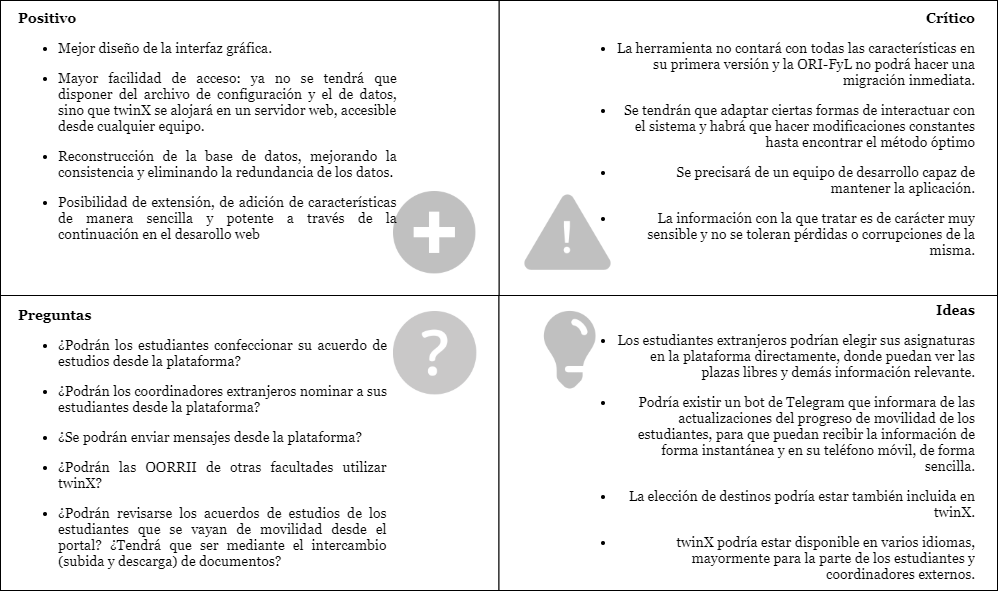
\includegraphics[width=\textwidth]{img/malla.png}
	\caption{Malla receptora de la información}
	\label{fig:malla}
\end{figure}


\section{Descripción de la propuesta}
Una vez hemos dado pinceladas de todo lo que tenemos, de qué podemos hacer, qué no y cómo llevarlo a cabo, vamos a establecer los claros objetivos de este proyecto y definir exactamente cuál será el producto tras su finalización, una vez conocemos todo el entorno que lo rodea. 

\subsection{Elección de la metodología de desarrollo}
Para desarrollar twinX primero se ha de elegir una metodología. Tradicionalmente, los proyectos de software se construían siguiendo lo que se conocen como «metodologías pesadas» o tradicionales \citep{waterfall1}, largos procesos de desarrollo en los que se definen unas fases secuenciales por donde el producto iba pasando hasta tener una versión final. La metodología más sonada es la de «cascada» o \textit{waterfall} en inglés \citep{waterfall2}. En ella, tenían lugar unas estrictas etapas enfocadas a un grupo de tareas en concreto, como son la etapa de definición, la de diseño, la de codificación, la de pruebas y la de mejora. Todo ello daba lugar a documentaciones muy completas aunque innecesariamente extensas en muchos casos, a través de la implicación de mucha gente experta en la materia, capacitada para hacer las tareas definidas muy concretamente. La flexibilidad apenas estaba contemplada, puesto que la planificación era muy estricta y hacía peligrar la buena continuidad del proyecto.

Hoy en día, apenas se utiliza este tipo de metodologías. En nuestro caso, queremos construir lo que sería tan sólo el comienzo del producto final. En otras palabras, nuestras condiciones no encajarían en una metodología en cascada, pues no tenemos unos requisitos estrictamente fijados, ya que vamos a crear una versión de TWINS no definitiva y la cual no se verá con todas las características implementadas. Además, es un cambio tan drástico el que se va a dar al transportar la aplicación a la web, que se precisa de la continua atención de una especie de «equipo supervisor», conformado por uno o varios usuarios finales del producto, que nos pueda proporcionar un \textit{feedback} sobre si nos estamos acercando o alejando de sus expectativas. Sobre esto último, diremos que no es que no se tuviera en cuenta en las metodologías tradicionales, pero no se primaba tanto como se debería, lo que hacía que el software perdiera calidad.

Por todo ello, podemos aventurarnos a decir que nuestro proyecto encaja más en una \textbf{metodología ágil}. Este tipo de metodologías se basan en la adaptación a medios con necesidades cambiantes, con un desarrollo muy de cerca con el cliente, quien está presente junto con el equipo de desarrollo en las numerosas reuniones que se hacen a lo largo de la vida del proyecto. Es más, en el \textit{14th Annual State of Agile Report} \citep{stateofagile} podemos encontrar unas estadísticas sobre los beneficios que ha traído el uso de metodologías ágiles en el último año, entre las que podemos destacar la capacidad de manejar los cambios de prioridades, la reducción de riesgos en el proyecto o el mantenimiento del software. En este caso, el equipo de desarrollo es ajustado, pero no por ello dejaremos de lado la necesaria intervención de dos personas fundamentales que hacen el papel de clientes y que son:

\begin{itemize}
	\item María Consuelo Pérez Ocaña (Coordinadora de Internacionalización en la la Facultad de Filosofía y Letras)
	\item Miguel Ángel Sanz Sáez (personal de secretaría y creador de TWINS)
\end{itemize}

\subsection{Propuesta de producto}
En su primera versión, twinX incluirá la funcionalidad mínima de TWINS, de modo que de cara a las pruebas, la interacción con la nueva plataforma sea más bien realista, y aporte verosimilitud a la mejora, pudiendo así ser tomada como tal.

Más concretamente, contemplamos la implementación de:

\begin{itemize}
	\item El añadido, modificación y eliminación de información esencial (como son asignaturas, tipo de expediente --similar a \gls{ExpedienteTWINS}--, mensajes predefinidos, etc.)
	\item La visualización de la información relevante a estudiantes (sus datos personales, expedientes abiertos, fases de los mismos, etc.)
	\item La visualización de los \glspl{Convenio}, modificación de la información y el añadido de nuevos. Posibilidad de dos vistas: una de resumen y otra completa, tal y como se tiene en TWINS.
	\item Calendario con eventos, tareas, tal y como se disponía en TWINS
	\item El envío de mensajes, a modo de sustituir los avisos en TWINS, pero abriendo el abanico a tres tipos de mensaje: mensaje normal, recordatorio (mensaje de un usuario para sí mismo) y avisos (por proximidad a la fecha de un evento o al límite para realizar una determinada tarea).
	\item Una pantalla inicial de visualización de la información de mayor relevancia a modo de resumen. 
	\item Organización de todo el contenido en tres grandes secciones: «gestión», «calendario» y «panel de control», para simplificar y mejorar la interfaz de usuario, facilitando la interacción con la misma.
\end{itemize}

\section{Presupuesto}

\section{Planificación}
